\chapter{Brief history of data science}
\label{chap:history}

\chapterprecishere{``Begin at the beginning,'' the King said gravely, ``and
go on till you come to the end: then stop.''\par\raggedleft--- \textup{Lewis
Carroll}, Alice in Wonderland}

There are many points-of-view about the beginning of data science.  For the sake of
contextualization, I separate the topic in two approaches: the history of the term itself
and a broad timeline of data-driven sciences highlighting the important figures in each
age.

I believe that the history of the term is important to understand the context of the
discipline.  Along the years, the term has been used to label rather different fields of
study.  Before I present my view on the term, I present the views of two important
figures in the history of data science: Peter Naur and William Cleveland.

Moreover, studying the main facts and figures in the history of data-driven sciences
enables us to understand the evolution of the field and hopefully to guide us to evolve it
further.  Most of the important theories and methods in data science have been developed
simultaneously in different fields, such as statistics, computer science, and engineering.
The history of data-driven sciences is long and rich. I present a timeline of the ages of
data handling and the most important markers of data analysis.

I do not intend to provide a comprehensive history of data science.  I aim to provide
enough context to support the development of the material in the following chapters,
sometimes avoiding directions that are not relevant in the inductive learning context.

\begin{mainbox}{Chapter remarks}

  \boxsubtitle{Contents}

  \startcontents[chapters]
  \printcontents[chapters]{}{1}{}
  \vspace{1em}

  \boxsubtitle{Context}

  \begin{itemize}
    \item The term ``data science'' is recent and has been used to label rather different
      fields.
    \item The history of data-driven sciences is long and rich.
    \item Many important theories and methods in data science have been developed
      simultaneously in different fields.
    \item The history of data-driven sciences is important to understand the evolution of
      the field.
  \end{itemize}

  \boxsubtitle{Objectives}

  \begin{itemize}
    \item Understand the history of the term ``data science.''
    \item Understand the major milestones in the history of data-driven sciences.
    \item Identify important figures in the history of data-driven sciences.
  \end{itemize}

  \boxsubtitle{Takeways}

  \begin{itemize}
    \item We have evolved both in terms of theory and application of data-driven sciences.
    \item There is no consensus on the definition of data science (including which fields
      it encompasses).
    \item However, there is enough evidence to support data science as a new science.
  \end{itemize}
\end{mainbox}

{}
\clearpage

\section{The term ``data science''}

The term data science is recent and has been used to label rather different fields of
study.  In the following, I emphasize the history of a few notable usage of the term.

\def\naurds{(0,0) circle (20mm)}
\def\naurcs{(0:5mm) circle (15mm)}
\def\naurde{(0:40mm) circle (15mm)}

\colorlet{circle edge}{black!50}
\colorlet{circle area}{black!20}

\tikzset{filled/.style={fill=circle area, draw=circle edge, thick},
    outline/.style={draw=circle edge, thick}}

\paragraph{Peter Naur (1928 -- 2016)}

The term ``data science'' itself was coined in the 1960s by Peter Naur (/naʊə/). Naur was
a Danish computer scientist and mathematician who made significant contributions to the
field of computer science, including his work on the development of programming
languages\footnote{He is best remembered as a contributor, with John Backus, to the
Backus–Naur form (BNF) notation used in describing the syntax for most programming
languages.}.
His ideas and concepts laid the groundwork for the way we think about programming and data
processing today.

% \begin{slidebox}{Peter Naur}{}
%   \begin{itemize}
%     \item Danish computer scientist and mathematician.
%     \item Coined the term ``data science'' in the 1960s.
%     \item Proposed the term ``datalogy'' as an alternative to computer science.
%   \end{itemize}
% \end{slidebox}

Naur disliked the term computer science and suggested it be called datalogy or data
science.  In the 1960s, the subject was practised in Denmark under Peter
Naur's term datalogy, which means the science of data and data processes.

He coined this term to emphasize the importance of data as a fundamental component of
computer science and to encourage a broader perspective on the field that included
data-related aspects. At that time, the field was primarily centered on programming
techniques, but Naur's concept broadened the scope to recognize the intrinsic role of data
in computation.

In his book\footfullcite{Naur1974}, ``Concise Survey of Computer Methods'', he
parts from the concept that \emph{data} is ``a representation of facts or ideas in a
formalised manner capable of being communicated or manipulated by some
process.''\footnote{I. H. Gould (ed.): ‘IFIP guide to concepts and terms in data
processing’, North-Holland Publ. Co., Amsterdam, 1971.} Note however that his view of the
science only ``deals with data [\dots] while the relation of data to what they represent
is delegated to other fields and sciences.''

\begin{figurebox}[label=fig:naur]{Naur's view of data science.}
  \centering
  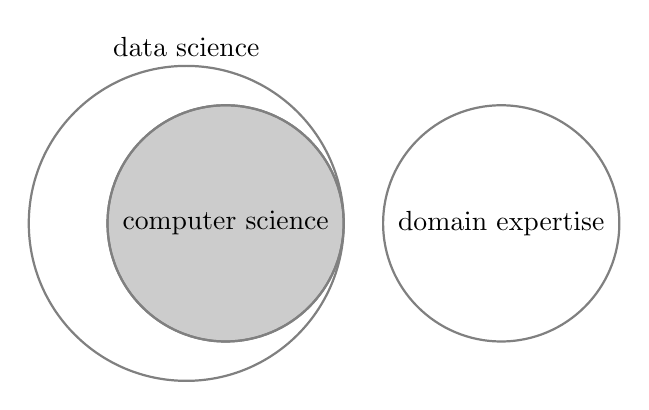
\begin{tikzpicture}
    \begin{scope}
      \clip \naurds;
      \fill[filled] \naurcs;
    \end{scope}
    \draw[outline] \naurds node(ds) {};
    \draw[outline] \naurcs node {computer science};
    \draw[outline] \naurde node {domain expertise};
    \node[anchor=north,above] at (0,2) {data science};
  \end{tikzpicture}
  \tcblower
    For Naur, data science studies the techniques to deal
    with data, but he delegates the meaning of data to other fields.
\end{figurebox}

It is interesting to see the central role he gave to data in the field of computer
science. His view that the relation of data to what they represent is delegated to other
fields and sciences is still debatable today.  Some scientists argue that data science
should focus on the techniques to deal with data, while others argue that data science
should encompass the whole business domain.  A depiction of Naur's view of data science is
shown in \cref{fig:naur}.

\def\clevelandds{(0,0) circle (20mm)}
\def\clevelandst{(0:-5mm) circle (15mm)}
\def\clevelandde {(2,1) circle (15mm)}
\def\clevelandcs {(2,-1) circle (15mm)}

\paragraph{William Cleveland (born 1943)}

In 2001, a prominent statistician used the term ``data science'' in his work to describe a
new discipline that comes from his ``plan to enlarge the major areas of technical work of
the field of statistics\footfullcite{Cleveland2001}.''
In 2014, that work was republished\footnote{W. S. Cleveland.
Data Science: An Action Plan for the Field of Statistics. Statistical Analysis and Data
Mining, 7:414–417, 2014. reprinting of 2001 article in ISI Review, Vol 69.}.
He advocates the expansion of statistics beyond theory into technical areas, significantly
changing statistics.  Thus, it warranted a new name.

% \begin{slidebox}{William Cleveland}{}
%   \begin{itemize}
%     \item American statistician.
%     \item Proposed the discipline ``data science'' in 2001.
%     \item Proposed the term ``data science'' as the new name for expansion of statistics.
%   \end{itemize}
% \end{slidebox}

As a result, William Swain Cleveland II is credited to define data science as it is most
used today. He is a highly influential figure in the fields of statistics, machine
learning, data visualization, data analysis for multidisciplinary studies, and high
performance computing for deep data analysis.

\begin{figurebox}[label=fig:cleveland]{Cleveland's view of data science.}
  \centering
  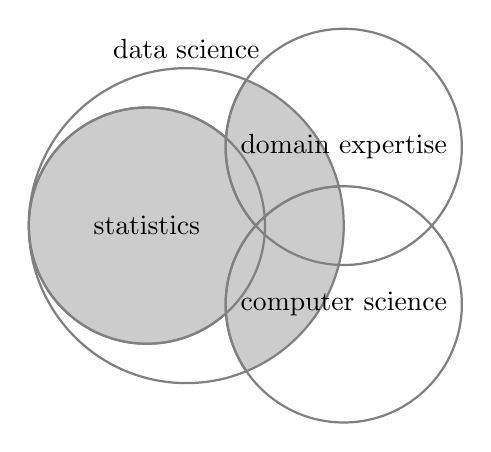
\begin{tikzpicture}
    \begin{scope}
      \clip \clevelandds;
      \fill[filled] \clevelandst;
      \fill[filled] \clevelandde;
      \fill[filled] \clevelandcs;
    \end{scope}
    \draw[outline] \clevelandds node(ds) {};
    \draw[outline] \clevelandst node {statistics};
    \draw[outline] \clevelandde node {domain expertise};
    \draw[outline] \clevelandcs node {computer science};
    \node[anchor=north,above] at (0,2) {data science};
  \end{tikzpicture}
  \tcblower
    For Cleveland, data science is the ``modern'' statistics,
    where it is enlarged by computer science and domain expertise.
\end{figurebox}

In his view, data science is the ``modern'' statistics, where it is enlarged by computer
science methods and domain expertise.  An illustration of Cleveland's view of data science
is shown in \cref{fig:cleveland}.  It is important to note that Cleveland never defined a
explicit list of computer science fields and business domains that should be included in
the new discipline.  The main idea is that statistics should rely on computational methods
and that the domain expertise should be considered in the analysis.

\paragraph{Buzzword or a new science?}

Be aware that scientific literature has no consensus on the definition of data science, and it is still considered
by some to be a buzzword\footnote{Press, Gil. ``Data Science: What's The Half-Life of a
Buzzword?''. Forbes. Available at
\url{https://www.forbes.com/sites/gilpress/2013/08/19/data-science-whats-the-half-life-of-a-buzzword/}}.

Most of the usages of the term in literature and in the media are either a rough
reference to a set of data-driven techniques or a marketing strategy.  Naur
(\cref{fig:naur}) and Cleveland (\cref{fig:cleveland}) are among the few that try to
carefully define the term.  However, both of them do not see data science as an
independent field of study, but an enlarged scope of an existing science.  I disagree;
the social and economical demand for data-driven solutions led to an evolution in our
understanding of the challenges we are facing.  As a result, we see many ``data
scientist'' being hired and many ``data science degrees'' programs emerging.

In \cref{chap:data}, I dare to provide a (yet another) definition for the term.  I
argue that its object of study can be precisely established to support it as a new
science.

% \begin{slidebox}{A new science}{}
%   \begin{itemize}
%     \item Both Naur and Cleveland do not see data science as an independent field of study.
%     \item I argue that data science is not a buzzword.
%     \item Our social and economical reality demands a new science.
%   \end{itemize}
% \end{slidebox}

\section{Timeline and historical markers}

\textcite{Kelleher2018} provides an interesting timeline of data-driven methods and
influential figures in the field.  I reproduce it here with some changes, including
some omissions and additions.  On the subject of data analysis, I include some of the
exceptional remarks
from \textcite{Vapnik1999b}.

I first address data handling --- which I include data sources, collection, organization,
storage, and transformation ---, and then data analysis and knowledge extraction.

\subsection{Timeline of data handling}

The importance of collecting and organizing data goes without saying.  Data fuels analysis and
decision making.  In the following, I present some of the most important milestones in the history
of data handling.

\begin{figurebox}[label=fig:data-handling-history]{Timeline of the ages of data handling.}
  \centering
  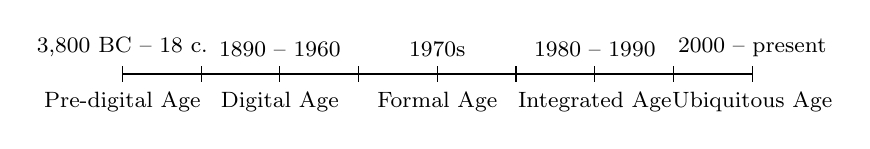
\begin{tikzpicture}
    \draw (0,0) -- (8,0);
    \foreach \x in {0,1,...,8} {
      \draw (\x,-0.1) -- (\x,0.1);
    }
    \foreach \x/\y/\z in {%
        0/Pre-digital Age/{3,800 BC -- \nth{18} c.},
        2/Digital Age/{1890 -- 1960},
        4/Formal Age/{1970s},
        6/Integrated Age/{1980 -- 1990},
        8/Ubiquitous Age/{2000 -- present}} {
      \node[anchor=north] at (\x,-0.1) {\footnotesize\y};
      \node[anchor=south] at (\x,0.1) {\footnotesize\z};
    }
  \end{tikzpicture}
\end{figurebox}

\Cref{fig:data-handling-history} illutrates the proposed timeline.  Ages are not strict
boundaries, but rather periods where some important events happened.  Also, observe that
the timescale is not linear.  The Pre-digital Age is the longest period, and one could
divide it into smaller periods.  My choices of ages and their boundaries are motivated by
didactic reasons.

\subsubsection{Pre-digital age}

We can consider the earliest records of data collection to be the notches on sticks and
bones to keep tracking of passing of time.  The Lebombo bone, a baboon fibula with
notches, is probably the earliest known mathematical object.  It was found in the Lebombo
Mountains located between South Africa and Eswatini.
They estimate it is more
than 40,000 years old. It is conjectured to be a tally stick, but its exact purpose is
unknown. Its 29 notches suggests that may have been used as a lunar phase counter.
However, since it is broken at one end, the 29 notches may or may not be the total
number\footfullcite{Beaumont2013}.

Another important milestone in the history of data collection is the record of
demographic data.  One of first known census was conducted in 3,800 BC in the Babylonian
Empire.  It was ordered to assess the population and resources of
his empire.  Records were stored on  clay  tiles\footfullcite{Grajalez2013}.

Since the early forms of writing, humanity abilities to record events and information
increased significantly.  The first known written records date back to around 3,500 BC, the
Sumerian archaic (pre-cuneiform) writing.  This writing system was used to represent
commodities using clay tokens and to record transactions\footfullcite{Ifrah1998}.

``Data storage'' was also a challenge.  Some important devices that increased our capacity
to register textual information are the Sumerian clay tablets (3,500 BC), the Egyptian
papyrus (3,000 BC), the Roman wax tablets (100 BC), the codex
(100 AD), the Chinese paper (200 AD), the printing press (1440), and the typewriter (1868).

% Talvez citar na parte de análise de dados
% Other mechanisms were also developed to store information in a more structured way.  Some
% important devices are
% the abacus (2,700 BC), the Antikythera mechanism (150 -- 100 BC), the
% Chinese South Pointing Chariot (260 AD), the Pascaline (1642), the Jacquard loom (1801),
% the Babbage Difference Engine (1822), the Babbage Analytical Engine (1837).

Besides those improvements in unstructured data storage, at least in the Western and
Middle Eastern world, there are no significant advances in structured data collection
until the \nth{19} century.  (A Eastern timeline research seems much hard to perform.
Unfortunally, I left it out in this book.)

I consider a major influential figure in the history of data
collection to be Florence Nightingale (1820 -- 1910).  She was a passionate statistician
and probably the first person to use statistics to influence public and official
opinion.  The meticulous records she kept during the Crimean War
(1853 -- 1856) were the evidence that saved lives --- part of the mortality came from lack
of sanitation.  She was also the first to use
statistical graphics to present data in a way that was easy to understand.  She is
credited with developing a form of the pie chart now known as the polar area
diagram.  She also reformed healthcare in the United Kingdom and
is considered the founder of modern nursing; where great part of the work was to collect
data in a standardized way to quickly draw conclusions\footfullcite{Grajalez2013}.

% \begin{slidebox}{Pre-digital age}{}
%   \begin{itemize}
%     \item Babylonian census (3,800 BC)
%     \item Sumerian archaic (pre-cuneiform) writing (3,500 BC)
%     \item Egyptian papyrus (3,000 BC)
%     \item Phoenician alphabet (1,000 BC)
%     \item Greek alphabet (800 BC)
%     \item Roman wax tablets (100 BC)
%     \item Codex (100 AD)
%     \item Chinese paper (200 AD)
%     \item Printing press (1440)
%     \item Typewriter (1868)
%     \item Florence Nightingale (1820 -- 1910)
%   \end{itemize}
% \end{slidebox}
%
% \begin{slidebox}{Florence Nightingale}{}
%   \begin{itemize}
%     \item Passionate statistician.
%     \item First person to use statistics to influence public and official opinion.
%     \item Organized data from garden fruits and vegetables into numerical tables at the age of 9.
%     \item At 20 she was receiving two-hour lessons from a Cambridge-trained mathematician.
%     \item She found the sight of a long column of figures ``perfectly reviving.''
%     \item She went out to the Crimean War, to Scutari in Turkey, in 1854.
%     \item She found that not even the numbers of soldiers entering the hospitals, or leaving them – alive or dead – was known.
%     \item From the first she kept meticulous records.
%     \item The data she collected was the evidence that saved lives.
%     \item She was the first to use statistical graphics to present data in a way that was easy to understand.
%     \item She is credited with developing a form of the pie chart now known as the polar area diagram.
%     \item She reformed healthcare in the United Kingdom and is considered the founder of modern nursing.
%   \end{itemize}
% \end{slidebox}

\subsubsection{Digital age}

In the modern period, several devices were developed to store digital\footnote{Digital
means the representation of information in (finite) discrete form.  The term comes from the Latin
digitus, meaning finger, because it is the natural way to count using fingers.  Digital
here do not mean electronic.}
information.  One particular device that is important for data collection is the punched
card.  It is a piece of stiff paper that contains digital information represented by the
presence or absence of holes in predefined positions.  The information can be read by a
mechanical or electrical device called a card reader.  The earliest famous usage of
punched cards was by Basile Bouchon (1725) to control looms.  Most of the advances until
the 1880s were about the automation of machines (data processing) using hand-punched cards, and not
particularly specialized for data collection.

However, the 1890 census in the United States was the first to use machine-readable
punched cards to tabulate data. Processing 1880 census data took eight years, so the
Census Bureau contracted Herman Hollerith (1860 -- 1929) to design and build a tabulating
machine.  He founded the Tabulating Machine Company in 1896, which later merged with other
companies to become International Business Machines Corporation (IBM) in 1924. Later
models of the tabulating machine were widely used for business applications such as
accounting and inventory control. Punched card technology remained a prevalent method of
data processing for several decades until more advanced electronic computers were
developed in the mid-\nth{20} century.

The invention of the digital computer is responsible for a revolution in data handling.
The amount of information we can capture and store increased exponentially.  ENIAC (1945) was
the first electronic general-purpose computer.  It was Turing-complete, digital, and
capable of being reprogrammed to solve a full range of computing problems.
It had 20 words of internal memory, each capable of storing a 10-digit decimal integer number.
Programs and data were entered by setting switches and inserting punched cards.

For the 1950 census, the United States Census Bureau used the
UNIVAC I (Universal Automatic Computer I), the first commercially produced computer in the
United States\footnote{Read more in \url{https://www.census.gov/history/www/innovations/}.}.

It goes without saying that digital computers have become much more powerful and
sophisticated since then.  The data collection process has been easily automated and
scaled to a level that was unimaginable before.  However, ``where'' storing data is
not the only challenge.  ``How'' to store data is also a challenge.  The next period of
history addresses this issue.

% \begin{slidebox}{Digital age}{}
%   \begin{itemize}
%     \item Punched card (1725)
%     \item 1890 census and Hollerith's tabulating machine (1890)
%     \item ENIAC (1945)
%     \item UNIVAC I used by the United Census Bureau (1950)
%   \end{itemize}
% \end{slidebox}

\subsubsection{Formal age}

In 1970, Edgar Frank Codd (1923 -- 2003), a British computer scientist,
published a paper entitled ``A Relational Model
of Data for Large Shared Data Banks''\footfullcite{Codd1970}.  In this paper, he introduced
the concept of a relational model for database management.

A relational model organizes data in tables (relations) where each row represents a record
and each column represents an attribute of the record.  The tables are related by common
fields.  Codd showed means to organize the tables of a relational database to minimize
data redundancy and improve data integrity.  \Cref{sec:normalization} provides more details
on the topic.

His work was a breakthrough in the field of data management.  The standardization of
relational databases led to the development of Structured Query Language (SQL) in 1974.
SQL is a domain-specific language used in programming and designed for managing data held
in a relational database management system (RDBMS).

As a result, a new challenge rapidly emerged: how to aggregate data from different
sources. Once data is stored in a relational database, it is easy to query and manage
it. However, data is usually stored in different databases, and it is not always possible
to directly combine them.

% \begin{slidebox}{Edgar Frank Codd}{}
%   \begin{itemize}
%     \item British computer scientist
%     \item Introduced the concept of a relational model for database management
%     \item Standardized relational databases
%     \item Led the development of Structured Query Language (SQL)
%   \end{itemize}
% \end{slidebox}

\subsubsection{Integrated age}

The solution to this problem was the development of the Extract, Transform, Load (ETL)
process.  ETL is a process in data warehousing responsible for extracting data from
several sources, transforming it into a format that can be analyzed, and loading it into a
data warehouse.

The concept of data warehousing dates back to the late 1980s when IBM researchers Barry
Devlin and Paul Murphy developed the ``business data warehouse.''

Two major figures in the history of ETL are Ralph Kimball (born 1944) and Bill Inmon (born
1945), both American computer scientists.  Although they
differ in their approaches, they both agree that data warehousing is the foundation for
business intelligence (BI) and analytics, and that data warehouses should be designed to
be easy to understand and fast to query for business users.

A famous debate between Kimball and Inmon is the top-down versus bottom-up approach to
data warehousing.  Inmon's approach is top-down, where the data warehouse is designed
first and then the data marts\footnote{A data mart is a specialized subset of a data
warehouse that is designed to serve the needs of a specific business unit, department, or
functional area within an organization.} are created from the data warehouse.  Kimball's
approach is bottom-up, where the data marts are created first and then the data warehouse
is created from the data marts.

% \begin{slidebox}{Ralph Kimball}{}
%   \begin{itemize}
%     \item American computer scientist.
%     \item Developed the bottom-up approach to data warehousing.
%     \item From available data marts, the data warehouse is created.
%   \end{itemize}
% \end{slidebox}
%
% \begin{slidebox}{Bill Inmon}{}
%   \begin{itemize}
%     \item American computer scientist.
%     \item Developed the top-down approach to data warehousing.
%     \item Design the data warehouse first and then the data marts are created from the data warehouse.
%   \end{itemize}
% \end{slidebox}

One of the earliest and most famous case studies of the implementation of a data warehouse
is that of Walmart. In the early 1990s, Walmart faced the challenge of managing and
analyzing vast amounts of data from its stores across the United States. The company
needed a solution that would enable comprehensive reporting and analysis to support
decision-making processes.  The solution was to implement a data warehouse that would
integrate data from various sources and provide a single source of truth for the
organization.

\subsubsection{Ubiquitous age}

The last and current period of history is the ubiquitous age.  It is characterized by the
proliferation of data sources.

The ubiquity of data generation and the evolution of data-centric technologies have been
made possible by a multitude of figures across various domains.

\begin{itemize}
  \item Tim Berners-Lee, credited with inventing the World Wide Web, laid the foundation
    for the massive data flow on the internet.
  \item Vinton Cerf and Robert Kahn, often referred to as the ``Fathers of the Internet,''
    developed the TCP/IP protocols, which are fundamental to internet communication.
  \item Steve Jobs and Steve Wozniak (Apple Inc.) and Bill Gates (Microsoft Corporation),
    the introduction of personal computers, leading to the democratization of data
    generation.
  \item Mark Zuckerberg, the co-founder of Facebook, played a crucial role in the rise of
    social media and the generation of vast amounts of user-generated content.
  \item Larry Page and Sergey Brin, the founders of Google, transformed how we access and
    search for information.
  \item Elon Musk and Tesla, the rise of the Internet of Things (IoT) and connected
    devices.
\end{itemize}

In terms of data handling, this change in the data landscape has brought about the
development of new technologies and techniques for data storage and processing.  Especially
the development of NoSQL databases and distributed computing frameworks.

NoSQL databases are non-relational databases that can store and process large volumes of
unstructured, semi-structured, and structured data.  They are highly scalable and
flexible, making them ideal for big data applications.

\begin{slidebox}{The V's of big data}{}
  \begin{itemize}
    \item Volume: The amount of data generated is massive
    \item Velocity: The speed at which data is generated is high
    \item Variety: The types of data generated are diverse
    \item Veracity: The quality of data generated is questionable
    \item Value: The value of data generated is high
  \end{itemize}
\end{slidebox}

Once massive amounts of unstructured data became available, the need for new data
processing techniques arose.  The development of distributed computing frameworks such as
Apache Hadoop and Apache Spark enabled the processing of massive amounts of data in a
distributed manner.

Doug Cutting and Mike Cafarella, the developers of Apache Hadoop, revolutionized big data
proposed the Hadoop Distributed File System (HDFS) and MapReduce, which are the
cornerstones of the Hadoop framework, in 2006.  Hadoop's distributed storage and
processing capabilities enabled organizations to handle and analyze massive volumes of
data.

Currently, Google holds a patent for
MapReduce\footnote{\url{http://static.googleusercontent.com/media/research.google.com/es/us/archive/mapreduce-osdi04.pdf}}.
However, their framework inherits from the architeture proposed in \textcite{Hillis1985}
thesis.

MapReduce is not particularly novel, but its simplicity and scalability made it popular.

Nowadays, another important topic is Internet of Things (IoT).  IoT is a system of
interrelated computing devices that communicate with each other over the internet.
The devices can be anything from cellphones, coffee makers, washing machines, headphones,
lamps, wearable devices, and almost anything else you can think of.  IoT increased the
challenges of data handling, especially in terms of data storage and processing.

\subsection{Timeline of data analysis}

The way we think about data and knowledge extraction has evolved significantly over the
years.  In the following, I present some of the most important milestones in the history
of data analysis.

\subsubsection{Summary statistics}

The earliest known records of systematic data analysis date back to the first censuses.
The term \emph{statistics} itself refer to the analysis of data \emph{about the state},
including demographics and economics.  That early (and simplest) form of statistical
analysis is called \emph{summary statistics}, which consists of describing data in terms
of its central tendencies (e.g. arithmetic mean) e variability (e.g. range).

\subsubsection{Probability advent}

However, after the seventeenth century, the foundations of modern probability theory were
laid out.  Important figures for developing the probability theory are Blaise Pascal (1623
-- 1662), Pierre de Fermat (1607 -- 1665), Christiaan Huygens (1629 -- 1695), and Jacob
Bernoulli (1655 -- 1705).

The foundation methods brought to life the field of statistical inference. In the
following years, important results were achieved.

\paragraph{Bayes' rule}

Reverend Thomas Bayes (1701 -- 1761) was an English statistician, philosopher, and
presbyterian minister.  He is known for formulating a specific case of the theorem that
bears his name: Bayes' theorem.  The theorem is used to calculate conditional
probabilities using an algorithm (his Proposition 9, published in 1763) that uses evidence to calculate
limits on an unknown parameter.

The Bayes' rule is the foundation of learning from evidence, once it allows us to
calculate the probability of an event based on prior knowledge of conditions that might be
related to the event.  Classifiers based on Naïve Bayes --- the application of Bayes'
theorem with strong independence assumptions between known variables --- is likely to have
been used since the second half of the eighteenth century.

\paragraph{Gauss' method of least squares}

Johann Carl Friedrich Gauss (1777 -- 1855) was a German mathematician and physicist who made
significant contributions to many fields in mathematics and sciences.  Circa 1794, he
developed the method of least squares for calculating the orbit of Ceres to minimize the
impact of measurement error\footnote{The method was first published by Adrien-Marie
Legendre (1752 -- 1833) in 1805, but Gauss claimed in 1809 that he
had been using it since circa 1794.}.

\paragraph{Playfair's data visualization}

William Playfair (1759 -- 1823) was a secret agent on behalf of Great Britain during its
war with France in the 1790s.  He invented several types of diagram between 1780s and
1800s, such as the line, area and bar chart of economic data, and the pie chart and circle
graph to show proportions.

\begin{slidebox}{Probability advent}{}
  \begin{itemize}
    \item Foundations by Blaise Pascal, Pierre de Fermat, Christiaan Huygens, Jacob
      Bernoulli, and others (\nth{17} century)
    \item Bayes' rule by Thomas Bayes (1763)
    \item Gauss' method of least squares by Johann Carl Friedrich Gauss (1794)
    \item Playfair's data visualization by William Playfair (1780s -- 1800s)
  \end{itemize}
\end{slidebox}

\subsubsection{Learning from data}

In the twentieth century and beyond, new advances were made in the field of statistics.  The
development of learning methods\footnote{Vapnik uses the terminology \emph{learning
machines}.} enabled the development of new techniques for
data analysis.

\paragraph{Fisher's discriminant analysis}

In the 1930s, Ronald Fisher (1890 -- 1962) developed discriminant analysis, which was
considered a problem of constructing a decision rule to assign a vector to one of two
categories using given probability distribution functions\footnote{After, Rosenblatt's work,
however, it was used to solve inductive inference as well.}.

See \cref{sub:fisher} for more details about the technique.

\paragraph{Shannon's information theory}

The field, that studies quantification, storage and communication of information, was
originally established by the works of Harry Nyquist (1889 -- 1976) and Ralph Hartley
(1888 -- 1970) in the 1920s, and Claude Shannon (1916 -- 2001) in the 1940s.
Information theory brought many important concepts to the field of data analysis, such as
entropy, mutual information, and information gain.

\paragraph{K-Nearest Neighbors}

In 1951, Evelyn Fix (1904 -- 1965) and Joseph Lawson Hodges Jr. (1922 -- 2000) wrote a
technical report entitled ``Discriminatory Analysis, Nonparametric Discrimination:
Consistency Properties.''  In this paper, they proposed the k-nearest neighbors algorithm,
which is a non-parametric method used for classification and regression.

See \cref{sub:knn} for more details about the technique.

\paragraph{Rosenblatt's perceptron}

In the 1960s, Frank Rosenblatt (1928 -- 1971) developed the perceptron, the first model of
a learning machine.  While the idea of a mathematical neuron was not new, he was the first
to describe the model as a program, showing the ability of the perceptron to learn simple
tasks such as the logical operations AND and OR.

See \cref{sub:perceptron} for more details about the technique.

\paragraph{Hunt inducing trees}

In 1966, \citeauthor{Hunt1966}'s book\footfullcite{Hunt1966} described a way to induce decision trees from
data.  The algorithm is based on the concept of information entropy and is a precursor of
the \citeauthor{Quinlan1986}'s ID3 algorithm\footfullcite{Quinlan1986} and its variations.

See \cref{sub:tree} for more details about the technique.

\begin{slidebox}{Learning from data (part I)}{}
  \begin{itemize}
    \item Fisher's discriminant analysis by Ronald Fisher (1930s)
    \item Shannon's information theory by Claude Shannon (1940s)
    \item K-Nearest Neighbors by Evelyn Fix and Joseph Lawson Hodges Jr. (1951)
    \item Rosenblatt's perceptron by Frank Rosenblatt (1960s)
    \item Hunt inducing trees by John Ross Quinlan (1966)
  \end{itemize}
\end{slidebox}

\paragraph{Empirical risk minimization principle}

Although many learning machines where developed until the 1960s, they did not advanced
significantly the understanding of the general problem of learning from data.  Between
1960s and 1986 --- before the backpropagation algorithm was proposed ---, the field of practical
data analysis was basically stagnant.  The main reason for that was the lack of a
theoretical framework to support the development of new learning machines.

However, these years were not completely unfruitful.  As early as 1968, Vladimir Vapnik (1936 -- )
and Alexey Chervonenkis (1938 -- 2014) developed the foundamental concepts of VC entropy
and VC dimension for the data classification problems.  As a result, a novel inductive
principle was proposed: the Empirical Risk Minimization (ERM) principle.
This principle is the foundation of statistical learning theory.

% \paragraph{Algorithmic complexity}
%
% Solomonoff, Kolmogorov, and Chaitin proposed the first learning model based on
% algorithmic complexity.

\paragraph{Resurgence of neural networks}

In 1986, researchers developed independently a method to optimize coefficients of a neural
network\footfullcite{LeCun1986,Rumelhart1986}.  The method is called backpropagation and
is the foundation of the resurgence of neural networks.

This rebirth of neural networks happened in a scenario very different from the 1960s.
The availability of data and computational power fueled a new approach to the problem of
learning from data.  The new approach preferred the use of simple algorithms and
intuitive models over theoretical models, fueling areas such as bioinspired computing and
evolutionary computation.

\paragraph{Ensembles}

Following the new approach, ensemble methods were developed.  Based on ideas of
boosting\footfullcite{Schapire1990} and bagging\footfullcite{Breiman1996}, ensemble
methods combine multiple learning machines to improve the performance of the individual
machines.  The most famous ensemble methods are random forests\footfullcite{Ho1995}.

\paragraph{Support vector machines}

In 1995, \citeauthor{Cortes1995} proposed the support vector machine (SVM) algorithm, a
learning machine based on the VC theory and the ERM principle.  Based on Cover's
theorem\footfullcite{Cover1965}, they developed a method that finds the optimal hyperplane
that separates two classes of data with the maximum margin in a high-dimensional space.
The resulting method led to practical and efficient learning machines.

\paragraph{Deep learning revolution}

Although the ideia of neural networks with multiple layers were around since the 1960s,
only in the late 2000s the field of deep learning caught the attention of the scientific
community by achieving state-of-the-art results in computer vision and natural language
processing.  Yoshua Bengio, Geoffrey
Hinton and Yann LeCun are recognized for their for conceptual and engineering
breakthroughs in the field, winning the 2018 Turing Award.

% \paragraph{Knowledge discovery in databases}
%
% 1990s, Fayyad, Piatesky-Shapiro, and Smyth.
% Developed the KDD process, which is the foundation of data mining.
% Data mining is the process of discovering patterns in large data sets involving methods at
% the intersection of machine learning, statistics, and database systems.

\paragraph{Generative deep models}

Nowadays, generative deep models are a hot topic in machine learning. They are a class of
statistical models that can generate new data instances. They are used in unsupervised
learning to discover hidden structures in unlabeled data (e.g. clustering), and in
supervised learning to generate new synthetic data instances.  The most famous generative
models are the generative transformers and generative adversarial networks.

\paragraph{LUSI learning theory}

In 2010s, Vapnik and Rauf Izmailov proposed the Learning Using Statistical Invariants
(LUSI) principle, which is an extension of the statistical learning theory.  The LUSI
theory is based on the concept of statistical invariants, which are properties of
the data that are preserved under transformations.  The theory is the foundation of the
learning from intelligent teachers paradigm.  They regard the LUSI theory as the
next step in the evolution of learning theory, calling it the ``complete statistical
theory of learning''.

\begin{slidebox}{Learning from data (part II)}{}
  \begin{itemize}
    \item Empirical risk minimization principle by Vladimir Vapnik and Alexey Chervonenkis (1968)
    \item Resurgence of neural networks (1986)
    \item Ensembles (1990s)
    \item Support vector machines by Vladimir Vapnik and Corinna Cortes (1995)
    \item Deep learning revolution (2000s)
    \item Generative models (2010s)
    \item LUSI learning theory by Vladimir Vapnik and Rauf Izmailov (2010s)
  \end{itemize}
\end{slidebox}
